
\section{Compléments\,: autres axes XPath}

\subsection{Parent}

% Parent

\begin{frame}{Quelques axes en exemple : \texttt{parent}}
\texttt{parent} : le parent du n{\oe}ud courant.

\bigskip

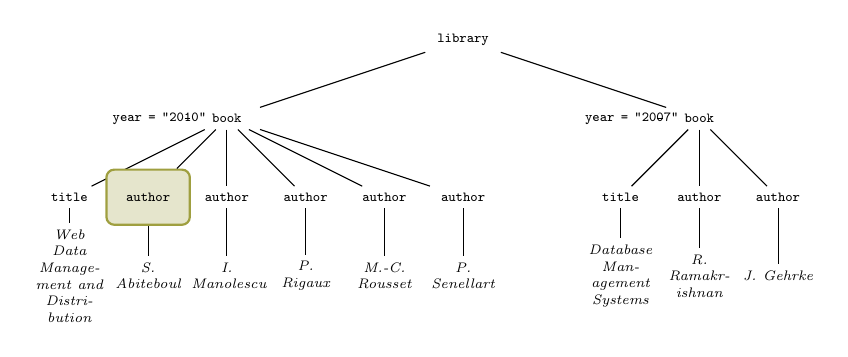
\begin{tikzpicture}[auto]
\tiny
  \tikzstyle{emptyStyle}=[text width=0.9cm, text centered]
  \tikzstyle{red}=[rounded corners=1mm,thick,draw=red!75,fill=red!20,text width=0.9cm, text centered]
  \tikzstyle{DarkViolet}=[rounded corners=1mm,thick,draw=DarkViolet!75,fill=DarkViolet!20,minimum size=7mm,text width=0.8cm, text centered]
  \tikzstyle{green}=[rounded corners=1mm,thick,draw=DarkOliveGreen!75,fill=DarkOliveGreen!20,minimum size=7mm,text width=0.8cm, text centered]
  \tikzstyle{cyan}=[rounded corners=1mm,thick,draw=DarkCyan!75,fill=DarkCyan!20,minimum size=7mm,text width=0.8cm, text centered]
 \tikzstyle{every label}=[black]
  \tikzstyle{HotPink}=[rounded corners=1mm,thick,draw=HotPink!75,fill=HotPink!20,minimum size=7mm,text width=0.8cm, text centered]
  \tikzstyle{noeudcourant}=[rounded corners=1mm,thick,draw=Olive!75,fill=Olive!20,minimum size=7mm,text width=0.9cm, text centered]
  \tikzstyle{indiaRed}=[rounded corners=1mm,thick,draw=indiaRed!75,fill=indiaRed!20,minimum size=7mm,text width=0.9cm, text centered]

  \begin{scope}
   % \node[emptyStyle](r) at (7,5) {Root};  
   %\node[emptyStyle](entete) at (3,4) {\texttt{$<?xml$ version $...>$}};
   %\draw[-] (r) -- (entete);
   \node[emptyStyle](library) at (7,4) {\verb?library?};
   % \draw[-] (r) -- (library);

    \node[emptyStyle](book1) at (4,3) {\verb?book?};
   \draw[-] (library) -- (book1);
   \node[emptyStyle](book2) at (10,3) {\verb?book?};
   \draw[-] (library) -- (book2);

    \node[emptyStyle](year1) at (3,3) {\verb?year = "2010"?};
   \draw[-] (book1) -- (year1);
    \node[emptyStyle](title1) at (2,2) {\verb?title?};
   \draw[-] (book1) -- (title1);
 \node[emptyStyle](texttitle1) at (2,1) {\it Web Data Management and Distribution};
   \draw[-] (title1) -- (texttitle1);
    \node[noeudcourant](author1) at (3,2) {\verb?author?};
   \draw[-] (book1) -- (author1);
   \node[emptyStyle](textauthor1) at (3,1) {\it S. Abiteboul};
   \draw[-] (author1) -- (textauthor1);
    \node[emptyStyle](author2) at (4,2) {\verb?author?};
   \draw[-] (book1) -- (author2);
   \node[emptyStyle](textauthor2) at (4,1) {\it I. Manolescu};
   \draw[-] (author2) -- (textauthor2);
    \node[emptyStyle](author3) at (5,2) {\verb?author?};
   \draw[-] (book1) -- (author3);
   \node[emptyStyle](textauthor3) at (5,1) {\it P. Rigaux};
   \draw[-] (author3) -- (textauthor3);
    \node[emptyStyle](author4) at (6,2) {\verb?author?};
   \draw[-] (book1) -- (author4);
   \node[emptyStyle](textauthor4) at (6,1) {\it M.-C. Rousset};
   \draw[-] (author4) -- (textauthor4);
    \node[emptyStyle](author5) at (7,2) {\verb?author?};
   \draw[-] (book1) -- (author5);
   \node[emptyStyle](textauthor5) at (7,1) {\it P. Senellart};
   \draw[-] (author5) -- (textauthor5);

    \node[emptyStyle](year2) at (9,3) {\verb?year = "2007"?};
   \draw[-] (book2) -- (year2);
    \node[emptyStyle](title2) at (9,2) {\verb?title?};
   \draw[-] (book2) -- (title2);
 \node[emptyStyle](texttitle2) at (9,1) {\it Database Management Systems};
   \draw[-] (title2) -- (texttitle2);
    \node[emptyStyle](author1prime) at (10,2) {\verb?author?};
   \draw[-] (book2) -- (author1prime);
   \node[emptyStyle](textauthor1prime) at (10,1) {\it R. Ramakrishnan};
   \draw[-] (author1prime) -- (textauthor1prime);
    \node[emptyStyle](author2prime) at (11,2) {\verb?author?};
   \draw[-] (book2) -- (author2prime);
   \node[emptyStyle](textauthor2prime) at (11,1) {\it J. Gehrke};
   \draw[-] (author2prime) -- (textauthor2prime);
\end{scope}
\end{tikzpicture}
\end{frame}


\begin{frame}{Quelques axes en exemple : \texttt{parent}}
\texttt{parent} : le parent du n{\oe}ud courant.

\bigskip

\begin{tikzpicture}[auto]
\tiny
  \tikzstyle{emptyStyle}=[text width=0.9cm, text centered]
  \tikzstyle{red}=[rounded corners=1mm,thick,draw=red!75,fill=red!20,text width=0.9cm, text centered]
  \tikzstyle{DarkViolet}=[rounded corners=1mm,thick,draw=DarkViolet!75,fill=DarkViolet!20,minimum size=7mm,text width=0.8cm, text centered]
  \tikzstyle{green}=[rounded corners=1mm,thick,draw=DarkOliveGreen!75,fill=DarkOliveGreen!20,minimum size=7mm,text width=0.8cm, text centered]
  \tikzstyle{cyan}=[rounded corners=1mm,thick,draw=DarkCyan!75,fill=DarkCyan!20,minimum size=7mm,text width=0.8cm, text centered]
 \tikzstyle{every label}=[black]
  \tikzstyle{HotPink}=[rounded corners=1mm,thick,draw=HotPink!75,fill=HotPink!20,minimum size=7mm,text width=0.8cm, text centered]
  \tikzstyle{noeudcourant}=[rounded corners=1mm,thick,draw=Olive!75,fill=Olive!20,minimum size=7mm,text width=0.9cm, text centered]
  \tikzstyle{indiaRed}=[rounded corners=1mm,thick,draw=indiaRed!75,fill=indiaRed!20,minimum size=7mm,text width=0.9cm, text centered]

  \begin{scope}
   % \node[emptyStyle](r) at (7,5) {Root};  
   %\node[emptyStyle](entete) at (3,4) {\texttt{$<?xml$ version $...>$}};
   %\draw[-] (r) -- (entete);
   \node[emptyStyle](library) at (7,4) {\verb?library?};
   % \draw[-] (r) -- (library);

    \node[indiaRed](book1) at (4,3) {\verb?book?};
   \draw[-] (library) -- (book1);
   \node[emptyStyle](book2) at (10,3) {\verb?book?};
   \draw[-] (library) -- (book2);

    \node[emptyStyle](year1) at (3,3) {\verb?year = "2010"?};
   \draw[-] (book1) -- (year1);
    \node[emptyStyle](title1) at (2,2) {\verb?title?};
   \draw[-] (book1) -- (title1);
 \node[emptyStyle](texttitle1) at (2,1) {\it Web Data Management and Distribution};
   \draw[-] (title1) -- (texttitle1);
    \node[noeudcourant](author1) at (3,2) {\verb?author?};
   \draw[-] (book1) -- (author1);
   \node[emptyStyle](textauthor1) at (3,1) {\it S. Abiteboul};
   \draw[-] (author1) -- (textauthor1);
    \node[emptyStyle](author2) at (4,2) {\verb?author?};
   \draw[-] (book1) -- (author2);
   \node[emptyStyle](textauthor2) at (4,1) {\it I. Manolescu};
   \draw[-] (author2) -- (textauthor2);
    \node[emptyStyle](author3) at (5,2) {\verb?author?};
   \draw[-] (book1) -- (author3);
   \node[emptyStyle](textauthor3) at (5,1) {\it P. Rigaux};
   \draw[-] (author3) -- (textauthor3);
    \node[emptyStyle](author4) at (6,2) {\verb?author?};
   \draw[-] (book1) -- (author4);
   \node[emptyStyle](textauthor4) at (6,1) {\it M.-C. Rousset};
   \draw[-] (author4) -- (textauthor4);
    \node[emptyStyle](author5) at (7,2) {\verb?author?};
   \draw[-] (book1) -- (author5);
   \node[emptyStyle](textauthor5) at (7,1) {\it P. Senellart};
   \draw[-] (author5) -- (textauthor5);

    \node[emptyStyle](year2) at (9,3) {\verb?year = "2007"?};
   \draw[-] (book2) -- (year2);
    \node[emptyStyle](title2) at (9,2) {\verb?title?};
   \draw[-] (book2) -- (title2);
 \node[emptyStyle](texttitle2) at (9,1) {\it Database Management Systems};
   \draw[-] (title2) -- (texttitle2);
    \node[emptyStyle](author1prime) at (10,2) {\verb?author?};
   \draw[-] (book2) -- (author1prime);
   \node[emptyStyle](textauthor1prime) at (10,1) {\it R. Ramakrishnan};
   \draw[-] (author1prime) -- (textauthor1prime);
    \node[emptyStyle](author2prime) at (11,2) {\verb?author?};
   \draw[-] (book2) -- (author2prime);
   \node[emptyStyle](textauthor2prime) at (11,1) {\it J. Gehrke};
   \draw[-] (author2prime) -- (textauthor2prime);
\end{scope}
\end{tikzpicture}
\end{frame}

\begin{frame}{Quelques axes en exemple : \texttt{parent}}
\texttt{parent} : le parent du n{\oe}ud courant.

\bigskip

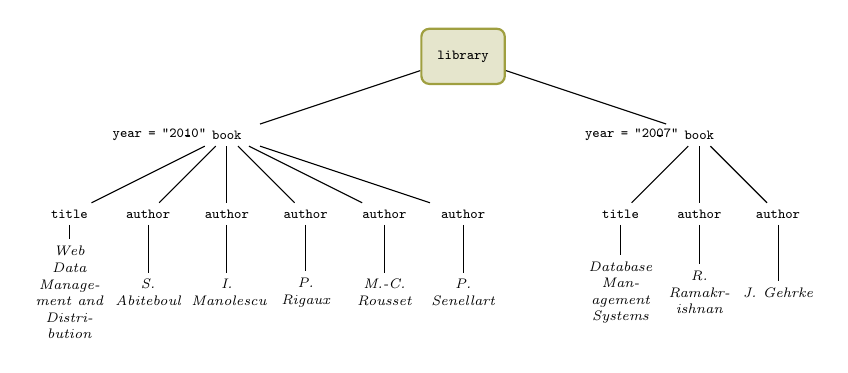
\begin{tikzpicture}[auto]
\tiny
  \tikzstyle{emptyStyle}=[text width=0.9cm, text centered]
  \tikzstyle{red}=[rounded corners=1mm,thick,draw=red!75,fill=red!20,text width=0.9cm, text centered]
  \tikzstyle{DarkViolet}=[rounded corners=1mm,thick,draw=DarkViolet!75,fill=DarkViolet!20,minimum size=7mm,text width=0.8cm, text centered]
  \tikzstyle{green}=[rounded corners=1mm,thick,draw=DarkOliveGreen!75,fill=DarkOliveGreen!20,minimum size=7mm,text width=0.8cm, text centered]
  \tikzstyle{cyan}=[rounded corners=1mm,thick,draw=DarkCyan!75,fill=DarkCyan!20,minimum size=7mm,text width=0.8cm, text centered]
 \tikzstyle{every label}=[black]
  \tikzstyle{HotPink}=[rounded corners=1mm,thick,draw=HotPink!75,fill=HotPink!20,minimum size=7mm,text width=0.8cm, text centered]
  \tikzstyle{noeudcourant}=[rounded corners=1mm,thick,draw=Olive!75,fill=Olive!20,minimum size=7mm,text width=0.9cm, text centered]
  \tikzstyle{indiaRed}=[rounded corners=1mm,thick,draw=indiaRed!75,fill=indiaRed!20,minimum size=7mm,text width=0.9cm, text centered]

  \begin{scope}
   % \node[emptyStyle](r) at (7,5) {Root};  
   %\node[emptyStyle](entete) at (3,4) {\texttt{$<?xml$ version $...>$}};
   %\draw[-] (r) -- (entete);
   \node[noeudcourant](library) at (7,4) {\verb?library?};
   % \draw[-] (r) -- (library);

    \node[emptyStyle](book1) at (4,3) {\verb?book?};
   \draw[-] (library) -- (book1);
   \node[emptyStyle](book2) at (10,3) {\verb?book?};
   \draw[-] (library) -- (book2);

    \node[emptyStyle](year1) at (3,3) {\verb?year = "2010"?};
   \draw[-] (book1) -- (year1);
    \node[emptyStyle](title1) at (2,2) {\verb?title?};
   \draw[-] (book1) -- (title1);
 \node[emptyStyle](texttitle1) at (2,1) {\it Web Data Management and Distribution};
   \draw[-] (title1) -- (texttitle1);
    \node[emptyStyle](author1) at (3,2) {\verb?author?};
   \draw[-] (book1) -- (author1);
   \node[emptyStyle](textauthor1) at (3,1) {\it S. Abiteboul};
   \draw[-] (author1) -- (textauthor1);
    \node[emptyStyle](author2) at (4,2) {\verb?author?};
   \draw[-] (book1) -- (author2);
   \node[emptyStyle](textauthor2) at (4,1) {\it I. Manolescu};
   \draw[-] (author2) -- (textauthor2);
    \node[emptyStyle](author3) at (5,2) {\verb?author?};
   \draw[-] (book1) -- (author3);
   \node[emptyStyle](textauthor3) at (5,1) {\it P. Rigaux};
   \draw[-] (author3) -- (textauthor3);
    \node[emptyStyle](author4) at (6,2) {\verb?author?};
   \draw[-] (book1) -- (author4);
   \node[emptyStyle](textauthor4) at (6,1) {\it M.-C. Rousset};
   \draw[-] (author4) -- (textauthor4);
    \node[emptyStyle](author5) at (7,2) {\verb?author?};
   \draw[-] (book1) -- (author5);
   \node[emptyStyle](textauthor5) at (7,1) {\it P. Senellart};
   \draw[-] (author5) -- (textauthor5);

    \node[emptyStyle](year2) at (9,3) {\verb?year = "2007"?};
   \draw[-] (book2) -- (year2);
    \node[emptyStyle](title2) at (9,2) {\verb?title?};
   \draw[-] (book2) -- (title2);
 \node[emptyStyle](texttitle2) at (9,1) {\it Database Management Systems};
   \draw[-] (title2) -- (texttitle2);
    \node[emptyStyle](author1prime) at (10,2) {\verb?author?};
   \draw[-] (book2) -- (author1prime);
   \node[emptyStyle](textauthor1prime) at (10,1) {\it R. Ramakrishnan};
   \draw[-] (author1prime) -- (textauthor1prime);
    \node[emptyStyle](author2prime) at (11,2) {\verb?author?};
   \draw[-] (book2) -- (author2prime);
   \node[emptyStyle](textauthor2prime) at (11,1) {\it J. Gehrke};
   \draw[-] (author2prime) -- (textauthor2prime);
\end{scope}
\end{tikzpicture}
\prof{Pas de n{\oe}ud parent}

\end{frame}


% ancestor
\subsection{Ancestor}

\begin{frame}{Quelques axes en exemple : \texttt{ancestor}}
\texttt{ancestor} : tous les ancêtres  (parent, grand-parent, etc.) du n{\oe}ud courant.

\bigskip

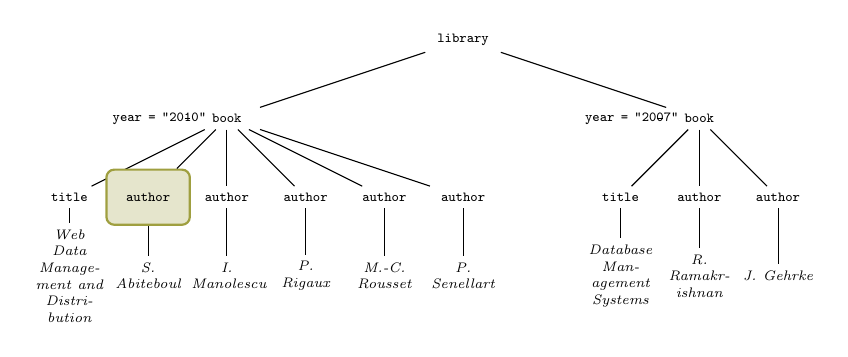
\begin{tikzpicture}[auto]
\tiny
  \tikzstyle{emptyStyle}=[text width=0.9cm, text centered]
  \tikzstyle{red}=[rounded corners=1mm,thick,draw=red!75,fill=red!20,text width=0.9cm, text centered]
  \tikzstyle{DarkViolet}=[rounded corners=1mm,thick,draw=DarkViolet!75,fill=DarkViolet!20,minimum size=7mm,text width=0.8cm, text centered]
  \tikzstyle{green}=[rounded corners=1mm,thick,draw=DarkOliveGreen!75,fill=DarkOliveGreen!20,minimum size=7mm,text width=0.8cm, text centered]
  \tikzstyle{cyan}=[rounded corners=1mm,thick,draw=DarkCyan!75,fill=DarkCyan!20,minimum size=7mm,text width=0.8cm, text centered]
 \tikzstyle{every label}=[black]
  \tikzstyle{HotPink}=[rounded corners=1mm,thick,draw=HotPink!75,fill=HotPink!20,minimum size=7mm,text width=0.8cm, text centered]
  \tikzstyle{noeudcourant}=[rounded corners=1mm,thick,draw=Olive!75,fill=Olive!20,minimum size=7mm,text width=0.9cm, text centered]
  \tikzstyle{indiaRed}=[rounded corners=1mm,thick,draw=indiaRed!75,fill=indiaRed!20,minimum size=7mm,text width=0.9cm, text centered]

  \begin{scope}
   % \node[emptyStyle](r) at (7,5) {Root};  
   %\node[emptyStyle](entete) at (3,4) {\texttt{$<?xml$ version $...>$}};
   %\draw[-] (r) -- (entete);
   \node[emptyStyle](library) at (7,4) {\verb?library?};
   % \draw[-] (r) -- (library);

    \node[emptyStyle](book1) at (4,3) {\verb?book?};
   \draw[-] (library) -- (book1);
   \node[emptyStyle](book2) at (10,3) {\verb?book?};
   \draw[-] (library) -- (book2);

    \node[emptyStyle](year1) at (3,3) {\verb?year = "2010"?};
   \draw[-] (book1) -- (year1);
    \node[emptyStyle](title1) at (2,2) {\verb?title?};
   \draw[-] (book1) -- (title1);
 \node[emptyStyle](texttitle1) at (2,1) {\it Web Data Management and Distribution};
   \draw[-] (title1) -- (texttitle1);
    \node[noeudcourant](author1) at (3,2) {\verb?author?};
   \draw[-] (book1) -- (author1);
   \node[emptyStyle](textauthor1) at (3,1) {\it S. Abiteboul};
   \draw[-] (author1) -- (textauthor1);
    \node[emptyStyle](author2) at (4,2) {\verb?author?};
   \draw[-] (book1) -- (author2);
   \node[emptyStyle](textauthor2) at (4,1) {\it I. Manolescu};
   \draw[-] (author2) -- (textauthor2);
    \node[emptyStyle](author3) at (5,2) {\verb?author?};
   \draw[-] (book1) -- (author3);
   \node[emptyStyle](textauthor3) at (5,1) {\it P. Rigaux};
   \draw[-] (author3) -- (textauthor3);
    \node[emptyStyle](author4) at (6,2) {\verb?author?};
   \draw[-] (book1) -- (author4);
   \node[emptyStyle](textauthor4) at (6,1) {\it M.-C. Rousset};
   \draw[-] (author4) -- (textauthor4);
    \node[emptyStyle](author5) at (7,2) {\verb?author?};
   \draw[-] (book1) -- (author5);
   \node[emptyStyle](textauthor5) at (7,1) {\it P. Senellart};
   \draw[-] (author5) -- (textauthor5);

    \node[emptyStyle](year2) at (9,3) {\verb?year = "2007"?};
   \draw[-] (book2) -- (year2);
    \node[emptyStyle](title2) at (9,2) {\verb?title?};
   \draw[-] (book2) -- (title2);
 \node[emptyStyle](texttitle2) at (9,1) {\it Database Management Systems};
   \draw[-] (title2) -- (texttitle2);
    \node[emptyStyle](author1prime) at (10,2) {\verb?author?};
   \draw[-] (book2) -- (author1prime);
   \node[emptyStyle](textauthor1prime) at (10,1) {\it R. Ramakrishnan};
   \draw[-] (author1prime) -- (textauthor1prime);
    \node[emptyStyle](author2prime) at (11,2) {\verb?author?};
   \draw[-] (book2) -- (author2prime);
   \node[emptyStyle](textauthor2prime) at (11,1) {\it J. Gehrke};
   \draw[-] (author2prime) -- (textauthor2prime);
\end{scope}
\end{tikzpicture}
\end{frame}


 \begin{frame}{Quelques axes en exemple : \texttt{ancestor}}
\texttt{ancestor} : tous les ancêtres  (parent, grand-parent, etc.) du n{\oe}ud courant.

\bigskip

\begin{tikzpicture}[auto]
\tiny
  \tikzstyle{emptyStyle}=[text width=0.9cm, text centered]
  \tikzstyle{red}=[rounded corners=1mm,thick,draw=red!75,fill=red!20,text width=0.9cm, text centered]
  \tikzstyle{DarkViolet}=[rounded corners=1mm,thick,draw=DarkViolet!75,fill=DarkViolet!20,minimum size=7mm,text width=0.8cm, text centered]
  \tikzstyle{green}=[rounded corners=1mm,thick,draw=DarkOliveGreen!75,fill=DarkOliveGreen!20,minimum size=7mm,text width=0.8cm, text centered]
  \tikzstyle{cyan}=[rounded corners=1mm,thick,draw=DarkCyan!75,fill=DarkCyan!20,minimum size=7mm,text width=0.8cm, text centered]
 \tikzstyle{every label}=[black]
  \tikzstyle{HotPink}=[rounded corners=1mm,thick,draw=HotPink!75,fill=HotPink!20,minimum size=7mm,text width=0.8cm, text centered]
  \tikzstyle{noeudcourant}=[rounded corners=1mm,thick,draw=Olive!75,fill=Olive!20,minimum size=7mm,text width=0.9cm, text centered]
  \tikzstyle{indiaRed}=[rounded corners=1mm,thick,draw=indiaRed!75,fill=indiaRed!20,minimum size=7mm,text width=0.9cm, text centered]

  \begin{scope}
   % \node[emptyStyle](r) at (7,5) {Root};  
   %\node[emptyStyle](entete) at (3,4) {\texttt{$<?xml$ version $...>$}};
   %\draw[-] (r) -- (entete);
   \node[indiaRed](library) at (7,4) {\verb?library?};
   % \draw[-] (r) -- (library);

    \node[indiaRed](book1) at (4,3) {\verb?book?};
   \draw[-] (library) -- (book1);
   \node[emptyStyle](book2) at (10,3) {\verb?book?};
   \draw[-] (library) -- (book2);

    \node[emptyStyle](year1) at (3,3) {\verb?year = "2010"?};
   \draw[-] (book1) -- (year1);
    \node[emptyStyle](title1) at (2,2) {\verb?title?};
   \draw[-] (book1) -- (title1);
 \node[emptyStyle](texttitle1) at (2,1) {\it Web Data Management and Distribution};
   \draw[-] (title1) -- (texttitle1);
    \node[noeudcourant](author1) at (3,2) {\verb?author?};
   \draw[-] (book1) -- (author1);
   \node[emptyStyle](textauthor1) at (3,1) {\it S. Abiteboul};
   \draw[-] (author1) -- (textauthor1);
    \node[emptyStyle](author2) at (4,2) {\verb?author?};
   \draw[-] (book1) -- (author2);
   \node[emptyStyle](textauthor2) at (4,1) {\it I. Manolescu};
   \draw[-] (author2) -- (textauthor2);
    \node[emptyStyle](author3) at (5,2) {\verb?author?};
   \draw[-] (book1) -- (author3);
   \node[emptyStyle](textauthor3) at (5,1) {\it P. Rigaux};
   \draw[-] (author3) -- (textauthor3);
    \node[emptyStyle](author4) at (6,2) {\verb?author?};
   \draw[-] (book1) -- (author4);
   \node[emptyStyle](textauthor4) at (6,1) {\it M.-C. Rousset};
   \draw[-] (author4) -- (textauthor4);
    \node[emptyStyle](author5) at (7,2) {\verb?author?};
   \draw[-] (book1) -- (author5);
   \node[emptyStyle](textauthor5) at (7,1) {\it P. Senellart};
   \draw[-] (author5) -- (textauthor5);

    \node[emptyStyle](year2) at (9,3) {\verb?year = "2007"?};
   \draw[-] (book2) -- (year2);
    \node[emptyStyle](title2) at (9,2) {\verb?title?};
   \draw[-] (book2) -- (title2);
 \node[emptyStyle](texttitle2) at (9,1) {\it Database Management Systems};
   \draw[-] (title2) -- (texttitle2);
    \node[emptyStyle](author1prime) at (10,2) {\verb?author?};
   \draw[-] (book2) -- (author1prime);
   \node[emptyStyle](textauthor1prime) at (10,1) {\it R. Ramakrishnan};
   \draw[-] (author1prime) -- (textauthor1prime);
    \node[emptyStyle](author2prime) at (11,2) {\verb?author?};
   \draw[-] (book2) -- (author2prime);
   \node[emptyStyle](textauthor2prime) at (11,1) {\it J. Gehrke};
   \draw[-] (author2prime) -- (textauthor2prime);
\end{scope}
\end{tikzpicture}
\end{frame}

\subsection{Ancestor-or-self}

 \begin{frame}{Quelques axes en exemple :\texttt{ancestor-or-self}}
\texttt{ancestor-or-self} : tous les ancêtres  (parent, grand-parent, etc.) du n{\oe}ud courant \alert{et} le n{\oe}ud courant
lui-même.

\bigskip

\begin{tikzpicture}[auto]
\tiny
  \tikzstyle{emptyStyle}=[text width=0.9cm, text centered]
  \tikzstyle{red}=[rounded corners=1mm,thick,draw=red!75,fill=red!20,text width=0.9cm, text centered]
  \tikzstyle{DarkViolet}=[rounded corners=1mm,thick,draw=DarkViolet!75,fill=DarkViolet!20,minimum size=7mm,text width=0.8cm, text centered]
  \tikzstyle{green}=[rounded corners=1mm,thick,draw=DarkOliveGreen!75,fill=DarkOliveGreen!20,minimum size=7mm,text width=0.8cm, text centered]
  \tikzstyle{cyan}=[rounded corners=1mm,thick,draw=DarkCyan!75,fill=DarkCyan!20,minimum size=7mm,text width=0.8cm, text centered]
 \tikzstyle{every label}=[black]
  \tikzstyle{HotPink}=[rounded corners=1mm,thick,draw=HotPink!75,fill=HotPink!20,minimum size=7mm,text width=0.8cm, text centered]
  \tikzstyle{noeudcourant}=[rounded corners=1mm,thick,draw=Olive!75,fill=Olive!20,minimum size=7mm,text width=0.9cm, text centered]
  \tikzstyle{indiaRed}=[rounded corners=1mm,thick,draw=indiaRed!75,fill=indiaRed!20,minimum size=7mm,text width=0.9cm, text centered]

  \begin{scope}
   % \node[emptyStyle](r) at (7,5) {Root};  
   %\node[emptyStyle](entete) at (3,4) {\texttt{$<?xml$ version $...>$}};
   %\draw[-] (r) -- (entete);
   \node[indiaRed](library) at (7,4) {\verb?library?};
   % \draw[-] (r) -- (library);

    \node[indiaRed](book1) at (4,3) {\verb?book?};
   \draw[-] (library) -- (book1);
   \node[emptyStyle](book2) at (10,3) {\verb?book?};
   \draw[-] (library) -- (book2);

    \node[emptyStyle](year1) at (3,3) {\verb?year = "2010"?};
   \draw[-] (book1) -- (year1);
    \node[emptyStyle](title1) at (2,2) {\verb?title?};
   \draw[-] (book1) -- (title1);
 \node[emptyStyle](texttitle1) at (2,1) {\it Web Data Management and Distribution};
   \draw[-] (title1) -- (texttitle1);
    \node[indiaRed](author1) at (3,2) {\verb?author?};
   \draw[-] (book1) -- (author1);
   \node[emptyStyle](textauthor1) at (3,1) {\it S. Abiteboul};
   \draw[-] (author1) -- (textauthor1);
    \node[emptyStyle](author2) at (4,2) {\verb?author?};
   \draw[-] (book1) -- (author2);
   \node[emptyStyle](textauthor2) at (4,1) {\it I. Manolescu};
   \draw[-] (author2) -- (textauthor2);
    \node[emptyStyle](author3) at (5,2) {\verb?author?};
   \draw[-] (book1) -- (author3);
   \node[emptyStyle](textauthor3) at (5,1) {\it P. Rigaux};
   \draw[-] (author3) -- (textauthor3);
    \node[emptyStyle](author4) at (6,2) {\verb?author?};
   \draw[-] (book1) -- (author4);
   \node[emptyStyle](textauthor4) at (6,1) {\it M.-C. Rousset};
   \draw[-] (author4) -- (textauthor4);
    \node[emptyStyle](author5) at (7,2) {\verb?author?};
   \draw[-] (book1) -- (author5);
   \node[emptyStyle](textauthor5) at (7,1) {\it P. Senellart};
   \draw[-] (author5) -- (textauthor5);

    \node[emptyStyle](year2) at (9,3) {\verb?year = "2007"?};
   \draw[-] (book2) -- (year2);
    \node[emptyStyle](title2) at (9,2) {\verb?title?};
   \draw[-] (book2) -- (title2);
 \node[emptyStyle](texttitle2) at (9,1) {\it Database Management Systems};
   \draw[-] (title2) -- (texttitle2);
    \node[emptyStyle](author1prime) at (10,2) {\verb?author?};
   \draw[-] (book2) -- (author1prime);
   \node[emptyStyle](textauthor1prime) at (10,1) {\it R. Ramakrishnan};
   \draw[-] (author1prime) -- (textauthor1prime);
    \node[emptyStyle](author2prime) at (11,2) {\verb?author?};
   \draw[-] (book2) -- (author2prime);
   \node[emptyStyle](textauthor2prime) at (11,1) {\it J. Gehrke};
   \draw[-] (author2prime) -- (textauthor2prime);
\end{scope}
\end{tikzpicture}


\prof{Exercice : ancestor et ancestor-or-self sur la biblio (racine)}
\end{frame}



\subsection{Descendant}
% descendant

\begin{frame}{Quelques axes en exemple : \texttt{descendant}}
\texttt{descendant} : tous les  descendants (enfants, petits-enfants, ) du n{\oe}ud courant.

\bigskip

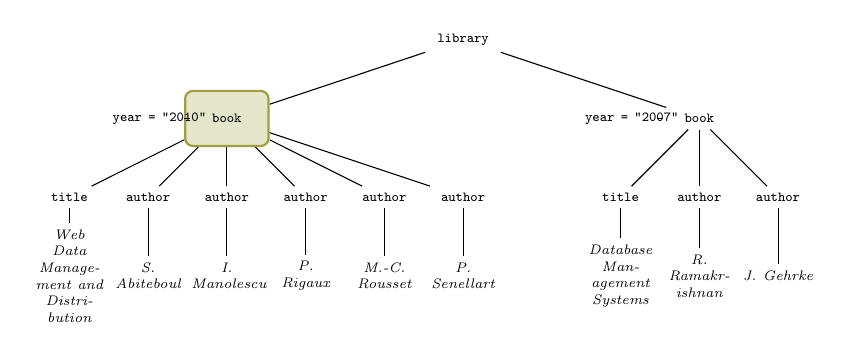
\begin{tikzpicture}[auto]
\tiny
  \tikzstyle{emptyStyle}=[text width=0.9cm, text centered]
  \tikzstyle{red}=[rounded corners=1mm,thick,draw=red!75,fill=red!20,text width=0.9cm, text centered]
  \tikzstyle{DarkViolet}=[rounded corners=1mm,thick,draw=DarkViolet!75,fill=DarkViolet!20,minimum size=7mm,text width=0.8cm, text centered]
  \tikzstyle{green}=[rounded corners=1mm,thick,draw=DarkOliveGreen!75,fill=DarkOliveGreen!20,minimum size=7mm,text width=0.8cm, text centered]
  \tikzstyle{cyan}=[rounded corners=1mm,thick,draw=DarkCyan!75,fill=DarkCyan!20,minimum size=7mm,text width=0.8cm, text centered]
 \tikzstyle{every label}=[black]
  \tikzstyle{HotPink}=[rounded corners=1mm,thick,draw=HotPink!75,fill=HotPink!20,minimum size=7mm,text width=0.8cm, text centered]
  \tikzstyle{noeudcourant}=[rounded corners=1mm,thick,draw=Olive!75,fill=Olive!20,minimum size=7mm,text width=0.9cm, text centered]
  \tikzstyle{indiaRed}=[rounded corners=1mm,thick,draw=indiaRed!75,fill=indiaRed!20,minimum size=7mm,text width=0.9cm, text centered]

  \begin{scope}
   % \node[emptyStyle](r) at (7,5) {Root};  
   %\node[emptyStyle](entete) at (3,4) {\texttt{$<?xml$ version $...>$}};
   %\draw[-] (r) -- (entete);
   \node[emptyStyle](library) at (7,4) {\verb?library?};
   % \draw[-] (r) -- (library);

    \node[noeudcourant](book1) at (4,3) {\verb?book?};
   \draw[-] (library) -- (book1);
   \node[emptyStyle](book2) at (10,3) {\verb?book?};
   \draw[-] (library) -- (book2);

    \node[emptyStyle](year1) at (3,3) {\verb?year = "2010"?};
   \draw[-] (book1) -- (year1);
    \node[emptyStyle](title1) at (2,2) {\verb?title?};
   \draw[-] (book1) -- (title1);
 \node[emptyStyle](texttitle1) at (2,1) {\it Web Data Management and Distribution};
   \draw[-] (title1) -- (texttitle1);
    \node[emptyStyle](author1) at (3,2) {\verb?author?};
   \draw[-] (book1) -- (author1);
   \node[emptyStyle](textauthor1) at (3,1) {\it S. Abiteboul};
   \draw[-] (author1) -- (textauthor1);
    \node[emptyStyle](author2) at (4,2) {\verb?author?};
   \draw[-] (book1) -- (author2);
   \node[emptyStyle](textauthor2) at (4,1) {\it I. Manolescu};
   \draw[-] (author2) -- (textauthor2);
    \node[emptyStyle](author3) at (5,2) {\verb?author?};
   \draw[-] (book1) -- (author3);
   \node[emptyStyle](textauthor3) at (5,1) {\it P. Rigaux};
   \draw[-] (author3) -- (textauthor3);
    \node[emptyStyle](author4) at (6,2) {\verb?author?};
   \draw[-] (book1) -- (author4);
   \node[emptyStyle](textauthor4) at (6,1) {\it M.-C. Rousset};
   \draw[-] (author4) -- (textauthor4);
    \node[emptyStyle](author5) at (7,2) {\verb?author?};
   \draw[-] (book1) -- (author5);
   \node[emptyStyle](textauthor5) at (7,1) {\it P. Senellart};
   \draw[-] (author5) -- (textauthor5);

    \node[emptyStyle](year2) at (9,3) {\verb?year = "2007"?};
   \draw[-] (book2) -- (year2);
    \node[emptyStyle](title2) at (9,2) {\verb?title?};
   \draw[-] (book2) -- (title2);
 \node[emptyStyle](texttitle2) at (9,1) {\it Database Management Systems};
   \draw[-] (title2) -- (texttitle2);
    \node[emptyStyle](author1prime) at (10,2) {\verb?author?};
   \draw[-] (book2) -- (author1prime);
   \node[emptyStyle](textauthor1prime) at (10,1) {\it R. Ramakrishnan};
   \draw[-] (author1prime) -- (textauthor1prime);
    \node[emptyStyle](author2prime) at (11,2) {\verb?author?};
   \draw[-] (book2) -- (author2prime);
   \node[emptyStyle](textauthor2prime) at (11,1) {\it J. Gehrke};
   \draw[-] (author2prime) -- (textauthor2prime);
\end{scope}
\end{tikzpicture}
\end{frame}


 \begin{frame}{Quelques axes en exemple : \texttt{descendant}}
\texttt{descendant} : tous les  descendants (enfants, petits-enfants, ) du n{\oe}ud courant.

\bigskip

\begin{tikzpicture}[auto]
\tiny
  \tikzstyle{emptyStyle}=[text width=0.9cm, text centered]
  \tikzstyle{red}=[rounded corners=1mm,thick,draw=red!75,fill=red!20,text width=0.9cm, text centered]
  \tikzstyle{DarkViolet}=[rounded corners=1mm,thick,draw=DarkViolet!75,fill=DarkViolet!20,minimum size=7mm,text width=0.8cm, text centered]
  \tikzstyle{green}=[rounded corners=1mm,thick,draw=DarkOliveGreen!75,fill=DarkOliveGreen!20,minimum size=7mm,text width=0.8cm, text centered]
  \tikzstyle{cyan}=[rounded corners=1mm,thick,draw=DarkCyan!75,fill=DarkCyan!20,minimum size=7mm,text width=0.8cm, text centered]
 \tikzstyle{every label}=[black]
  \tikzstyle{HotPink}=[rounded corners=1mm,thick,draw=HotPink!75,fill=HotPink!20,minimum size=7mm,text width=0.8cm, text centered]
  \tikzstyle{noeudcourant}=[rounded corners=1mm,thick,draw=Olive!75,fill=Olive!20,minimum size=7mm,text width=0.9cm, text centered]
  \tikzstyle{indiaRed}=[rounded corners=1mm,thick,draw=indiaRed!75,fill=indiaRed!20,minimum size=7mm,text width=0.9cm, text centered]

  \begin{scope}
   % \node[emptyStyle](r) at (7,5) {Root};  
   %\node[emptyStyle](entete) at (3,4) {\texttt{$<?xml$ version $...>$}};
   %\draw[-] (r) -- (entete);
   \node[emptyStyle](library) at (7,4) {\verb?library?};
   % \draw[-] (r) -- (library);

    \node[noeudcourant](book1) at (4,3) {\verb?book?};
   \draw[-] (library) -- (book1);
   \node[emptyStyle](book2) at (10,3) {\verb?book?};
   \draw[-] (library) -- (book2);

    \node[emptyStyle](year1) at (3,3) {\verb?year = "2010"?};
   \draw[-] (book1) -- (year1);
    \node[indiaRed](title1) at (2,2) {\verb?title?};
   \draw[-] (book1) -- (title1);
 \node[indiaRed](texttitle1) at (2,1) {\it Web Data Management and Distribution};
   \draw[-] (title1) -- (texttitle1);
    \node[indiaRed](author1) at (3,2) {\verb?author?};
   \draw[-] (book1) -- (author1);
   \node[indiaRed](textauthor1) at (3,1) {\it S. Abiteboul};
   \draw[-] (author1) -- (textauthor1);
    \node[indiaRed](author2) at (4,2) {\verb?author?};
   \draw[-] (book1) -- (author2);
   \node[indiaRed](textauthor2) at (4,1) {\it I. Manolescu};
   \draw[-] (author2) -- (textauthor2);
    \node[indiaRed](author3) at (5,2) {\verb?author?};
   \draw[-] (book1) -- (author3);
   \node[indiaRed](textauthor3) at (5,1) {\it P. Rigaux};
   \draw[-] (author3) -- (textauthor3);
    \node[indiaRed](author4) at (6,2) {\verb?author?};
   \draw[-] (book1) -- (author4);
   \node[indiaRed](textauthor4) at (6,1) {\it M.-C. Rousset};
   \draw[-] (author4) -- (textauthor4);
    \node[indiaRed](author5) at (7,2) {\verb?author?};
   \draw[-] (book1) -- (author5);
   \node[indiaRed](textauthor5) at (7,1) {\it P. Senellart};
   \draw[-] (author5) -- (textauthor5);

    \node[emptyStyle](year2) at (9,3) {\verb?year = "2007"?};
   \draw[-] (book2) -- (year2);
    \node[emptyStyle](title2) at (9,2) {\verb?title?};
   \draw[-] (book2) -- (title2);
 \node[emptyStyle](texttitle2) at (9,1) {\it Database Management Systems};
   \draw[-] (title2) -- (texttitle2);
    \node[emptyStyle](author1prime) at (10,2) {\verb?author?};
   \draw[-] (book2) -- (author1prime);
   \node[emptyStyle](textauthor1prime) at (10,1) {\it R. Ramakrishnan};
   \draw[-] (author1prime) -- (textauthor1prime);
    \node[emptyStyle](author2prime) at (11,2) {\verb?author?};
   \draw[-] (book2) -- (author2prime);
   \node[emptyStyle](textauthor2prime) at (11,1) {\it J. Gehrke};
   \draw[-] (author2prime) -- (textauthor2prime);
\end{scope}
\end{tikzpicture}
\end{frame}


\subsection{Descendant-or-self}

\begin{frame}{Quelques axes en exemple : \texttt{descendant-or-self}}
\texttt{descendant-or-self} : tous les  descendants (enfants, petits-enfants, ) du n{\oe}ud courant et le n{\oe}ud courant lui-même.
\bigskip

\begin{tikzpicture}[auto]
\tiny
  \tikzstyle{emptyStyle}=[text width=0.9cm, text centered]
  \tikzstyle{red}=[rounded corners=1mm,thick,draw=red!75,fill=red!20,text width=0.9cm, text centered]
  \tikzstyle{DarkViolet}=[rounded corners=1mm,thick,draw=DarkViolet!75,fill=DarkViolet!20,minimum size=7mm,text width=0.8cm, text centered]
  \tikzstyle{green}=[rounded corners=1mm,thick,draw=DarkOliveGreen!75,fill=DarkOliveGreen!20,minimum size=7mm,text width=0.8cm, text centered]
  \tikzstyle{cyan}=[rounded corners=1mm,thick,draw=DarkCyan!75,fill=DarkCyan!20,minimum size=7mm,text width=0.8cm, text centered]
 \tikzstyle{every label}=[black]
  \tikzstyle{HotPink}=[rounded corners=1mm,thick,draw=HotPink!75,fill=HotPink!20,minimum size=7mm,text width=0.8cm, text centered]
  \tikzstyle{noeudcourant}=[rounded corners=1mm,thick,draw=Olive!75,fill=Olive!20,minimum size=7mm,text width=0.9cm, text centered]
  \tikzstyle{indiaRed}=[rounded corners=1mm,thick,draw=indiaRed!75,fill=indiaRed!20,minimum size=7mm,text width=0.9cm, text centered]

  \begin{scope}
   % \node[emptyStyle](r) at (7,5) {Root};  
   %\node[emptyStyle](entete) at (3,4) {\texttt{$<?xml$ version $...>$}};
   %\draw[-] (r) -- (entete);
   \node[emptyStyle](library) at (7,4) {\verb?library?};
   % \draw[-] (r) -- (library);

    \node[indiaRed](book1) at (4,3) {\verb?book?};
   \draw[-] (library) -- (book1);
   \node[emptyStyle](book2) at (10,3) {\verb?book?};
   \draw[-] (library) -- (book2);

    \node[emptyStyle](year1) at (3,3) {\verb?year = "2010"?};
   \draw[-] (book1) -- (year1);
    \node[indiaRed](title1) at (2,2) {\verb?title?};
   \draw[-] (book1) -- (title1);
 \node[indiaRed](texttitle1) at (2,1) {\it Web Data Management and Distribution};
   \draw[-] (title1) -- (texttitle1);
    \node[indiaRed](author1) at (3,2) {\verb?author?};
   \draw[-] (book1) -- (author1);
   \node[indiaRed](textauthor1) at (3,1) {\it S. Abiteboul};
   \draw[-] (author1) -- (textauthor1);
    \node[indiaRed](author2) at (4,2) {\verb?author?};
   \draw[-] (book1) -- (author2);
   \node[indiaRed](textauthor2) at (4,1) {\it I. Manolescu};
   \draw[-] (author2) -- (textauthor2);
    \node[indiaRed](author3) at (5,2) {\verb?author?};
   \draw[-] (book1) -- (author3);
   \node[indiaRed](textauthor3) at (5,1) {\it P. Rigaux};
   \draw[-] (author3) -- (textauthor3);
    \node[indiaRed](author4) at (6,2) {\verb?author?};
   \draw[-] (book1) -- (author4);
   \node[indiaRed](textauthor4) at (6,1) {\it M.-C. Rousset};
   \draw[-] (author4) -- (textauthor4);
    \node[indiaRed](author5) at (7,2) {\verb?author?};
   \draw[-] (book1) -- (author5);
   \node[indiaRed](textauthor5) at (7,1) {\it P. Senellart};
   \draw[-] (author5) -- (textauthor5);

    \node[emptyStyle](year2) at (9,3) {\verb?year = "2007"?};
   \draw[-] (book2) -- (year2);
    \node[emptyStyle](title2) at (9,2) {\verb?title?};
   \draw[-] (book2) -- (title2);
 \node[emptyStyle](texttitle2) at (9,1) {\it Database Management Systems};
   \draw[-] (title2) -- (texttitle2);
    \node[emptyStyle](author1prime) at (10,2) {\verb?author?};
   \draw[-] (book2) -- (author1prime);
   \node[emptyStyle](textauthor1prime) at (10,1) {\it R. Ramakrishnan};
   \draw[-] (author1prime) -- (textauthor1prime);
    \node[emptyStyle](author2prime) at (11,2) {\verb?author?};
   \draw[-] (book2) -- (author2prime);
   \node[emptyStyle](textauthor2prime) at (11,1) {\it J. Gehrke};
   \draw[-] (author2prime) -- (textauthor2prime);
\end{scope}
\end{tikzpicture}

\end{frame}


\subsection{Following}
%following

 \begin{frame}{Quelques axes en exemple : \texttt{following}}
\texttt{following} : tous les n{\oe}uds du document \alert{après} le n{\oe}ud courant (dans un parcours pré-ordre).

\bigskip

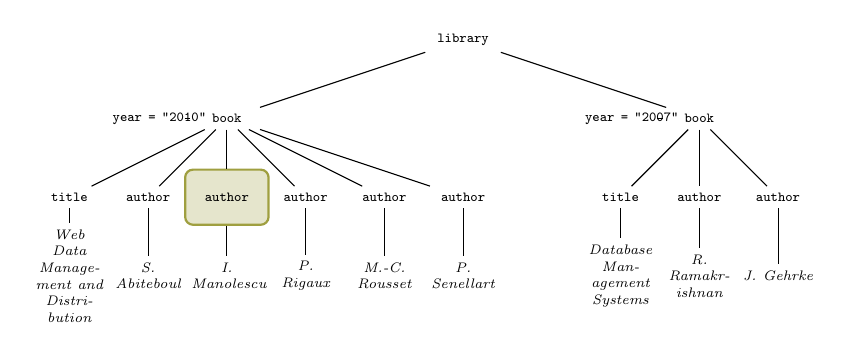
\begin{tikzpicture}[auto]
\tiny
  \tikzstyle{emptyStyle}=[text width=0.9cm, text centered]
  \tikzstyle{red}=[rounded corners=1mm,thick,draw=red!75,fill=red!20,text width=0.9cm, text centered]
  \tikzstyle{DarkViolet}=[rounded corners=1mm,thick,draw=DarkViolet!75,fill=DarkViolet!20,minimum size=7mm,text width=0.8cm, text centered]
  \tikzstyle{green}=[rounded corners=1mm,thick,draw=DarkOliveGreen!75,fill=DarkOliveGreen!20,minimum size=7mm,text width=0.8cm, text centered]
  \tikzstyle{cyan}=[rounded corners=1mm,thick,draw=DarkCyan!75,fill=DarkCyan!20,minimum size=7mm,text width=0.8cm, text centered]
 \tikzstyle{every label}=[black]
  \tikzstyle{HotPink}=[rounded corners=1mm,thick,draw=HotPink!75,fill=HotPink!20,minimum size=7mm,text width=0.8cm, text centered]
  \tikzstyle{noeudcourant}=[rounded corners=1mm,thick,draw=Olive!75,fill=Olive!20,minimum size=7mm,text width=0.9cm, text centered]
  \tikzstyle{indiaRed}=[rounded corners=1mm,thick,draw=indiaRed!75,fill=indiaRed!20,minimum size=7mm,text width=0.9cm, text centered]

  \begin{scope}
   % \node[emptyStyle](r) at (7,5) {Root};  
   %\node[emptyStyle](entete) at (3,4) {\texttt{$<?xml$ version $...>$}};
   %\draw[-] (r) -- (entete);
   \node[emptyStyle](library) at (7,4) {\verb?library?};
   % \draw[-] (r) -- (library);

    \node[emptyStyle](book1) at (4,3) {\verb?book?};
   \draw[-] (library) -- (book1);
   \node[emptyStyle](book2) at (10,3) {\verb?book?};
   \draw[-] (library) -- (book2);

    \node[emptyStyle](year1) at (3,3) {\verb?year = "2010"?};
   \draw[-] (book1) -- (year1);
    \node[emptyStyle](title1) at (2,2) {\verb?title?};
   \draw[-] (book1) -- (title1);
 \node[emptyStyle](texttitle1) at (2,1) {\it Web Data Management and Distribution};
   \draw[-] (title1) -- (texttitle1);
    \node[emptyStyle](author1) at (3,2) {\verb?author?};
   \draw[-] (book1) -- (author1);
   \node[emptyStyle](textauthor1) at (3,1) {\it S. Abiteboul};
   \draw[-] (author1) -- (textauthor1);
    \node[noeudcourant](author2) at (4,2) {\verb?author?};
   \draw[-] (book1) -- (author2);
   \node[emptyStyle](textauthor2) at (4,1) {\it I. Manolescu};
   \draw[-] (author2) -- (textauthor2);
    \node[emptyStyle](author3) at (5,2) {\verb?author?};
   \draw[-] (book1) -- (author3);
   \node[emptyStyle](textauthor3) at (5,1) {\it P. Rigaux};
   \draw[-] (author3) -- (textauthor3);
    \node[emptyStyle](author4) at (6,2) {\verb?author?};
   \draw[-] (book1) -- (author4);
   \node[emptyStyle](textauthor4) at (6,1) {\it M.-C. Rousset};
   \draw[-] (author4) -- (textauthor4);
    \node[emptyStyle](author5) at (7,2) {\verb?author?};
   \draw[-] (book1) -- (author5);
   \node[emptyStyle](textauthor5) at (7,1) {\it P. Senellart};
   \draw[-] (author5) -- (textauthor5);

    \node[emptyStyle](year2) at (9,3) {\verb?year = "2007"?};
   \draw[-] (book2) -- (year2);
    \node[emptyStyle](title2) at (9,2) {\verb?title?};
   \draw[-] (book2) -- (title2);
 \node[emptyStyle](texttitle2) at (9,1) {\it Database Management Systems};
   \draw[-] (title2) -- (texttitle2);
    \node[emptyStyle](author1prime) at (10,2) {\verb?author?};
   \draw[-] (book2) -- (author1prime);
   \node[emptyStyle](textauthor1prime) at (10,1) {\it R. Ramakrishnan};
   \draw[-] (author1prime) -- (textauthor1prime);
    \node[emptyStyle](author2prime) at (11,2) {\verb?author?};
   \draw[-] (book2) -- (author2prime);
   \node[emptyStyle](textauthor2prime) at (11,1) {\it J. Gehrke};
   \draw[-] (author2prime) -- (textauthor2prime);
\end{scope}
\end{tikzpicture}

\end{frame}

\begin{frame}{Quelques axes en exemple : Following}
\texttt{following}  : Selects everything in the document defined after the closing tag of the current node

\bigskip

\begin{tikzpicture}[auto]
\tiny
  \tikzstyle{emptyStyle}=[text width=0.9cm, text centered]
  \tikzstyle{red}=[rounded corners=1mm,thick,draw=red!75,fill=red!20,text width=0.9cm, text centered]
  \tikzstyle{DarkViolet}=[rounded corners=1mm,thick,draw=DarkViolet!75,fill=DarkViolet!20,minimum size=7mm,text width=0.8cm, text centered]
  \tikzstyle{green}=[rounded corners=1mm,thick,draw=DarkOliveGreen!75,fill=DarkOliveGreen!20,minimum size=7mm,text width=0.8cm, text centered]
  \tikzstyle{cyan}=[rounded corners=1mm,thick,draw=DarkCyan!75,fill=DarkCyan!20,minimum size=7mm,text width=0.8cm, text centered]
 \tikzstyle{every label}=[black]
  \tikzstyle{HotPink}=[rounded corners=1mm,thick,draw=HotPink!75,fill=HotPink!20,minimum size=7mm,text width=0.8cm, text centered]
  \tikzstyle{noeudcourant}=[rounded corners=1mm,thick,draw=Olive!75,fill=Olive!20,minimum size=7mm,text width=0.9cm, text centered]
  \tikzstyle{indiaRed}=[rounded corners=1mm,thick,draw=indiaRed!75,fill=indiaRed!20,minimum size=7mm,text width=0.9cm, text centered]

  \begin{scope}
   % \node[emptyStyle](r) at (7,5) {Root};  
   %\node[emptyStyle](entete) at (3,4) {\texttt{$<?xml$ version $...>$}};
   %\draw[-] (r) -- (entete);
   \node[emptyStyle](library) at (7,4) {\verb?library?};
   % \draw[-] (r) -- (library);

    \node[emptyStyle](book1) at (4,3) {\verb?book?};
   \draw[-] (library) -- (book1);
   \node[indiaRed](book2) at (10,3) {\verb?book?};
   \draw[-] (library) -- (book2);

    \node[emptyStyle](year1) at (3,3) {\verb?year = "2010"?};
   \draw[-] (book1) -- (year1);
    \node[emptyStyle](title1) at (2,2) {\verb?title?};
   \draw[-] (book1) -- (title1);
 \node[emptyStyle](texttitle1) at (2,1) {\it Web Data Management and Distribution};
   \draw[-] (title1) -- (texttitle1);
    \node[emptyStyle](author1) at (3,2) {\verb?author?};
   \draw[-] (book1) -- (author1);
   \node[emptyStyle](textauthor1) at (3,1) {\it S. Abiteboul};
   \draw[-] (author1) -- (textauthor1);
    \node[noeudcourant](author2) at (4,2) {\verb?author?};
   \draw[-] (book1) -- (author2);
   \node[emptyStyle](textauthor2) at (4,1) {\it I. Manolescu};
   \draw[-] (author2) -- (textauthor2);
    \node[indiaRed](author3) at (5,2) {\verb?author?};
   \draw[-] (book1) -- (author3);
   \node[indiaRed](textauthor3) at (5,1) {\it P. Rigaux};
   \draw[-] (author3) -- (textauthor3);
    \node[indiaRed](author4) at (6,2) {\verb?author?};
   \draw[-] (book1) -- (author4);
   \node[indiaRed](textauthor4) at (6,1) {\it M.-C. Rousset};
   \draw[-] (author4) -- (textauthor4);
    \node[indiaRed](author5) at (7,2) {\verb?author?};
   \draw[-] (book1) -- (author5);
   \node[indiaRed](textauthor5) at (7,1) {\it P. Senellart};
   \draw[-] (author5) -- (textauthor5);

    \node[indiaRed](year2) at (9,3) {\verb?year = "2007"?};
   \draw[-] (book2) -- (year2);
    \node[indiaRed](title2) at (9,2) {\verb?title?};
   \draw[-] (book2) -- (title2);
 \node[indiaRed](texttitle2) at (9,1) {\it Database Management Systems};
   \draw[-] (title2) -- (texttitle2);
    \node[indiaRed](author1prime) at (10,2) {\verb?author?};
   \draw[-] (book2) -- (author1prime);
   \node[indiaRed](textauthor1prime) at (10,1) {\it R. Ramakrishnan};
   \draw[-] (author1prime) -- (textauthor1prime);
    \node[indiaRed](author2prime) at (11,2) {\verb?author?};
   \draw[-] (book2) -- (author2prime);
   \node[indiaRed](textauthor2prime) at (11,1) {\it J. Gehrke};
   \draw[-] (author2prime) -- (textauthor2prime);
\end{scope}
\end{tikzpicture}

\end{frame}


%following-sibling
\subsection{Following-sibling}

 \begin{frame}{Quelques axes en exemple : Following-sibling}
\texttt{following-sibling} : Selects all siblings after the current node. \prof{sibling=frére ou s{\oe}ur}

\bigskip

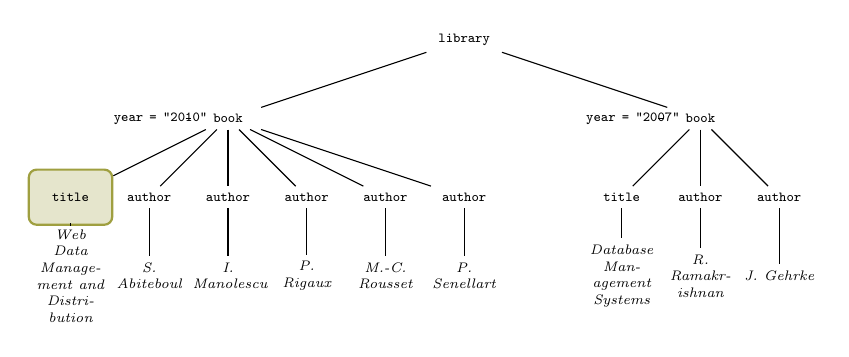
\begin{tikzpicture}[auto]
\tiny
  \tikzstyle{emptyStyle}=[text width=0.9cm, text centered]
  \tikzstyle{red}=[rounded corners=1mm,thick,draw=red!75,fill=red!20,text width=0.9cm, text centered]
  \tikzstyle{DarkViolet}=[rounded corners=1mm,thick,draw=DarkViolet!75,fill=DarkViolet!20,minimum size=7mm,text width=0.8cm, text centered]
  \tikzstyle{green}=[rounded corners=1mm,thick,draw=DarkOliveGreen!75,fill=DarkOliveGreen!20,minimum size=7mm,text width=0.8cm, text centered]
  \tikzstyle{cyan}=[rounded corners=1mm,thick,draw=DarkCyan!75,fill=DarkCyan!20,minimum size=7mm,text width=0.8cm, text centered]
 \tikzstyle{every label}=[black]
  \tikzstyle{HotPink}=[rounded corners=1mm,thick,draw=HotPink!75,fill=HotPink!20,minimum size=7mm,text width=0.8cm, text centered]
  \tikzstyle{noeudcourant}=[rounded corners=1mm,thick,draw=Olive!75,fill=Olive!20,minimum size=7mm,text width=0.9cm, text centered]
  \tikzstyle{indiaRed}=[rounded corners=1mm,thick,draw=indiaRed!75,fill=indiaRed!20,minimum size=7mm,text width=0.9cm, text centered]

  \begin{scope}
   % \node[emptyStyle](r) at (7,5) {Root};  
   %\node[emptyStyle](entete) at (3,4) {\texttt{$<?xml$ version $...>$}};
   %\draw[-] (r) -- (entete);
   \node[emptyStyle](library) at (7,4) {\verb?library?};
   % \draw[-] (r) -- (library);

    \node[emptyStyle](book1) at (4,3) {\verb?book?};
   \draw[-] (library) -- (book1);
   \node[emptyStyle](book2) at (10,3) {\verb?book?};
   \draw[-] (library) -- (book2);

    \node[emptyStyle](year1) at (3,3) {\verb?year = "2010"?};
   \draw[-] (book1) -- (year1);
    \node[noeudcourant](title1) at (2,2) {\verb?title?};
   \draw[-] (book1) -- (title1);
 \node[emptyStyle](texttitle1) at (2,1) {\it Web Data Management and Distribution};
   \draw[-] (title1) -- (texttitle1);
    \node[emptyStyle](author1) at (3,2) {\verb?author?};
   \draw[-] (book1) -- (author1);
   \node[emptyStyle](textauthor1) at (3,1) {\it S. Abiteboul};
   \draw[-] (author1) -- (textauthor1);
    \node[emptyStyle](author2) at (4,2) {\verb?author?};
   \draw[-] (book1) -- (author2);
   \node[emptyStyle](textauthor2) at (4,1) {\it I. Manolescu};
   \draw[-] (author2) -- (textauthor2);
    \node[emptyStyle](author3) at (5,2) {\verb?author?};
   \draw[-] (book1) -- (author3);
   \node[emptyStyle](textauthor3) at (5,1) {\it P. Rigaux};
   \draw[-] (author3) -- (textauthor3);
    \node[emptyStyle](author4) at (6,2) {\verb?author?};
   \draw[-] (book1) -- (author4);
   \node[emptyStyle](textauthor4) at (6,1) {\it M.-C. Rousset};
   \draw[-] (author4) -- (textauthor4);
    \node[emptyStyle](author5) at (7,2) {\verb?author?};
   \draw[-] (book1) -- (author5);
   \node[emptyStyle](textauthor5) at (7,1) {\it P. Senellart};
   \draw[-] (author5) -- (textauthor5);

    \node[emptyStyle](year2) at (9,3) {\verb?year = "2007"?};
   \draw[-] (book2) -- (year2);
    \node[emptyStyle](title2) at (9,2) {\verb?title?};
   \draw[-] (book2) -- (title2);
 \node[emptyStyle](texttitle2) at (9,1) {\it Database Management Systems};
   \draw[-] (title2) -- (texttitle2);
    \node[emptyStyle](author1prime) at (10,2) {\verb?author?};
   \draw[-] (book2) -- (author1prime);
   \node[emptyStyle](textauthor1prime) at (10,1) {\it R. Ramakrishnan};
   \draw[-] (author1prime) -- (textauthor1prime);
    \node[emptyStyle](author2prime) at (11,2) {\verb?author?};
   \draw[-] (book2) -- (author2prime);
   \node[emptyStyle](textauthor2prime) at (11,1) {\it J. Gehrke};
   \draw[-] (author2prime) -- (textauthor2prime);
\end{scope}
\end{tikzpicture}




\end{frame}


 \begin{frame}{Quelques axes en exemple : Following-sibling}
\texttt{following-sibling} : Selects all siblings after the current node

\bigskip

\begin{tikzpicture}[auto]
\tiny
  \tikzstyle{emptyStyle}=[text width=0.9cm, text centered]
  \tikzstyle{red}=[rounded corners=1mm,thick,draw=red!75,fill=red!20,text width=0.9cm, text centered]
  \tikzstyle{DarkViolet}=[rounded corners=1mm,thick,draw=DarkViolet!75,fill=DarkViolet!20,minimum size=7mm,text width=0.8cm, text centered]
  \tikzstyle{green}=[rounded corners=1mm,thick,draw=DarkOliveGreen!75,fill=DarkOliveGreen!20,minimum size=7mm,text width=0.8cm, text centered]
  \tikzstyle{cyan}=[rounded corners=1mm,thick,draw=DarkCyan!75,fill=DarkCyan!20,minimum size=7mm,text width=0.8cm, text centered]
 \tikzstyle{every label}=[black]
  \tikzstyle{HotPink}=[rounded corners=1mm,thick,draw=HotPink!75,fill=HotPink!20,minimum size=7mm,text width=0.8cm, text centered]
  \tikzstyle{noeudcourant}=[rounded corners=1mm,thick,draw=Olive!75,fill=Olive!20,minimum size=7mm,text width=0.9cm, text centered]
  \tikzstyle{indiaRed}=[rounded corners=1mm,thick,draw=indiaRed!75,fill=indiaRed!20,minimum size=7mm,text width=0.9cm, text centered]

  \begin{scope}
   % \node[emptyStyle](r) at (7,5) {Root};  
   %\node[emptyStyle](entete) at (3,4) {\texttt{$<?xml$ version $...>$}};
   %\draw[-] (r) -- (entete);
   \node[emptyStyle](library) at (7,4) {\verb?library?};
   % \draw[-] (r) -- (library);

    \node[emptyStyle](book1) at (4,3) {\verb?book?};
   \draw[-] (library) -- (book1);
   \node[emptyStyle](book2) at (10,3) {\verb?book?};
   \draw[-] (library) -- (book2);

    \node[emptyStyle](year1) at (3,3) {\verb?year = "2010"?};
   \draw[-] (book1) -- (year1);
    \node[noeudcourant](title1) at (2,2) {\verb?title?};
   \draw[-] (book1) -- (title1);
 \node[emptyStyle](texttitle1) at (2,1) {\it Web Data Management and Distribution};
   \draw[-] (title1) -- (texttitle1);
    \node[indiaRed](author1) at (3,2) {\verb?author?};
   \draw[-] (book1) -- (author1);
   \node[emptyStyle](textauthor1) at (3,1) {\it S. Abiteboul};
   \draw[-] (author1) -- (textauthor1);
    \node[indiaRed](author2) at (4,2) {\verb?author?};
   \draw[-] (book1) -- (author2);
   \node[emptyStyle](textauthor2) at (4,1) {\it I. Manolescu};
   \draw[-] (author2) -- (textauthor2);
    \node[indiaRed](author3) at (5,2) {\verb?author?};
   \draw[-] (book1) -- (author3);
   \node[emptyStyle](textauthor3) at (5,1) {\it P. Rigaux};
   \draw[-] (author3) -- (textauthor3);
    \node[indiaRed](author4) at (6,2) {\verb?author?};
   \draw[-] (book1) -- (author4);
   \node[emptyStyle](textauthor4) at (6,1) {\it M.-C. Rousset};
   \draw[-] (author4) -- (textauthor4);
    \node[indiaRed](author5) at (7,2) {\verb?author?};
   \draw[-] (book1) -- (author5);
   \node[emptyStyle](textauthor5) at (7,1) {\it P. Senellart};
   \draw[-] (author5) -- (textauthor5);

    \node[emptyStyle](year2) at (9,3) {\verb?year = "2007"?};
   \draw[-] (book2) -- (year2);
    \node[emptyStyle](title2) at (9,2) {\verb?title?};
   \draw[-] (book2) -- (title2);
 \node[emptyStyle](texttitle2) at (9,1) {\it Database Management Systems};
   \draw[-] (title2) -- (texttitle2);
    \node[emptyStyle](author1prime) at (10,2) {\verb?author?};
   \draw[-] (book2) -- (author1prime);
   \node[emptyStyle](textauthor1prime) at (10,1) {\it R. Ramakrishnan};
   \draw[-] (author1prime) -- (textauthor1prime);
    \node[emptyStyle](author2prime) at (11,2) {\verb?author?};
   \draw[-] (book2) -- (author2prime);
   \node[emptyStyle](textauthor2prime) at (11,1) {\it J. Gehrke};
   \draw[-] (author2prime) -- (textauthor2prime);
\end{scope}
\end{tikzpicture}

\end{frame}



\begin{frame}{Abréviations}

\textcolor{cyan}{\verb?child?} peut \^etre omis dans le chemin de localisation\\

\begin{flushright}
\textcolor{DarkViolet}{\verb?/inventory/drink/lemonade[child::amount>15]?}
\end{flushright}


\textcolor{cyan}{\verb?//a?} est une forme raccourcie de \textcolor{cyan}{\verb?/descendant-or-self::node()/child::a?}\\
\begin{flushright}
\textcolor{DarkViolet}{\verb?//lemonade[child::amount>15]?\\
\verb?/inventory//lemonade[child::amount>15]?}
\end{flushright}


\textcolor{cyan}{\verb?a//b?} est un raccourci pour \textcolor{cyan}{\verb?a/descendant-or-self::node()/child::b?}\\

\bigskip

\textcolor{cyan}{\verb?.?} est un raccourci pour \textcolor{cyan}{\verb?self::node()?}\\

\begin{flushright}
\textcolor{DarkViolet}{\verb?./inventory//lemonade[child::amount>15]?}
\end{flushright}

\textcolor{cyan}{\verb?..?} est un raccourci pour \textcolor{cyan}{\verb?parent::node()?}\\

\begin{flushright}
\textcolor{DarkViolet}{\verb?/inventory/drink/lemonade[child::amount>15]/../pop?}
\end{flushright}

\textcolor{cyan}{\verb?@attr\_name?} est un raccourci pour \textcolor{cyan}{\verb?attribute::attr\_name?}\\

\begin{flushright}
\textcolor{DarkViolet}{\verb?/inventory/drink/lemonade[@supplier='store']?}
\end{flushright}

\textcolor{cyan}{\verb?[1]?} est un raccourci pour \textcolor{cyan}{\verb?[position()=1]?}

\begin{flushright}
\textcolor{DarkViolet}{\verb?/inventory/drink[2]?}
\end{flushright}

\end{frame}

\begin{frame}[allowframebreaks]{Opérations et fonctions}

\begin{itemize}
\item XPath permet aussi d'effectuer des calculs des nombres, des booléens et des cha\^{i}nes de caractéres.

\item Opérations sur les nombres : \verb?+?, \verb?-? , \verb?*?, \verb?div?, \verb? mod?\\ \prof{Div au lieu de /, pourquoi ? Parce que / est un caractére spécial du langage utilisé pour les expressions de chemin
Modulo : le modulo est une fonction informatique qui au couple (a, b) d'entiers associe le reste r de la division euclidienne de a par b.}

Renvoie \verb?NaN? si l'un des arguments n'est pas un nombre. \prof{Not a Number}

\item Opérations sur les booléeans : \verb?and?, \verb?or?

\item égalité et différence (cha\^{i}nes de caractéres, nombres et booléens)  \verb?=?, \verb?!=? \prof{ex: \verb?@attr=1?}

\item Autres comparaisons (nombres seulement) : \verb?<?, \verb?<=?, \verb?>?, \verb?>= ?

\end{itemize}

\framebreak

{\bf Fonctions sur les ensembles de n{\oe}uds}
\begin{itemize}
\item \verb?count(nset)? nombre d'éléments dans l'ensemble de n{\oe}uds. 
\item \verb?name(nset)? nom du premier élément avec le préfixe de l'espace de noms
\item \verb?localname(nset)? nom du premier élément sans le préfixe de l'espace de noms
\item \verb?namespace-uri(nset)? préfixe de l'espace de noms du premier élément 
\item \verb?sum(nset)? somme des arguments de l'ensemble de n{\oe}uds (aprés conversion des cha\^{i}nes de caractéres en nombres).
\item \verb?position()? position dans le context
\item \verb?last()? nombre correspondant à la derniére position dans le context
\item \verb?id(mon\_id)? renvoi l'élément du document ayant pour identifiant \verb?mon\_id? (cherché parmis tous les attributs déclarés de type ID).
\end{itemize}

\begin{flushright}
\textcolor{DarkViolet}{\verb?//book[count(auteur)>=1]?\\
\verb?/biblio/book[position()=last()]?}
\end{flushright}

\framebreak

{\bf Fonctions sur les cha\^{i}nes de caractéres}

\begin{itemize}
\item \verb?concat(ch1, ..., chn)?, \verb?starts-with(ch1,ch2)?, \verb?contains(ch1,ch2)?, \verb?substring-before(ch1,ch2)?, \verb?substring-after(ch1,ch2)?, \verb?substring(ch,i,l)?, \verb?string-length(ch)?, \verb?normalize-space(ch)?, \verb?translate(ch1,ch2,ch3)?
\end{itemize}

\begin{flushright}
\textcolor{DarkViolet}{\verb?//titre[contains(text(),"Star")]?}
\end{flushright}

\prof{Exemple substring : extraire le ISBN 10  partir du ISBN 13.}

Voir \url{http://www.w3.org/TR/xpath\#section-Function-Calls}


\framebreak

{\bf Fonctions sur les booléens}

\begin{itemize}
\item \verb?not(bool)?
\end{itemize}

\begin{flushright}
\textcolor{DarkViolet}{\verb?not(@attr = 1)?\\
\verb?not(not(@attr = 1) or false()) and true()?\\
\verb?//book[not(count(auteur)>=1)]?
}
\end{flushright}


\framebreak

{\bf Fonctions sur les nombres}

\begin{itemize}
\item \verb?floor(n)? arrondi à l'entier supérieur de n
\item \verb?ceiling(n)? arrondi à l'entier inférieur de n
\item \verb?round(n)? arrondi entier de \verb?n? (plus proche de \verb?floor(n)? ou \verb?ceiling(n)?)
\end{itemize}

Voir \url{http://www.w3.org/TR/xpath\#section-Function-Calls}

\end{frame}


\begin{frame}{Zoom sur les espaces de noms}

\texttt{
<\textcolor{cyan}{html} xmlns="\textcolor{orange}{http://www.w3.org/1999/xhtml}">
</\textcolor{cyan}{html}>
}

\bigskip

Deux fonctions :\\
\textcolor{cyan}{local-name}\\
\textcolor{orange}{namespace-uri}\\

\bigskip

Utilisation (exemples) :\\
\verb?//*[local-name()='html']?\\
\verb?//*[namespace-uri()='http://www.w3.org/1999/xhtml'?\\
\verb?//*[local-name()='html']/namespace-uri()?\\

\end{frame}


\begin{frame}[allowframebreaks]{Zoom sur le cas des \texttt{ID} et \texttt{IDREF(S)}}

Fonctions :\\
id\\
idref\\

\bigskip

Utilisation (exemple) :\\

\verb?//id("0-201-53771-0")/child::author?	retourne les auteurs de l'élément dont l'ID est "0-201-53771-0"\\

\medskip

\verb?/library/document[3]/id(@references)/titre? retourne les titres des documents référencés (references est un IDREFS) par le troisième document\\

\medskip

\verb?//idref("0-201-53771-0")?	retourne tous les éléments qui référencent "0-201-53771-0"

\framebreak


\begin{center}
\figSized{images/exID1.jpg}{Fichier contenant des ID}{1}
\end{center}

\framebreak


\begin{center}
\figSized{images/exID2.jpg}{Requ\^ete avec fonction ID}{1}
\end{center}

\end{frame}

\begin{frame}{XPath 2.0}

 \begin{itemize}
 \item Repose toujours sur la notion de chemin de localisation afin de naviguer dans le document XML.
\item Pas juste une extension de XPath 1.0, c'est une véritable refonte de XPath : une fusion entre XPath 1.0 et XQuery.
\item Caractéristiques :
\begin{itemize}
\item Support de 19 types prédéfinis (date, etc), avec test de type ;
\item Réponse = séquence ordonnée de valeurs (et plus un NodeSet) ; \prof{ordonnée et autorisant les doublons à la place d'ensembles}
\item Opérateur d'intersection, union et except ;
\item Opérateurs de quantification ;
\item Boucles, tri, définition interne (let) ;
\item Expressions conditionnelles (if-then-else) ;
\item Extensible (possibilité de créer des fonctions utilisateurs).
\end{itemize}
 \end{itemize}

 $\Rightarrow$ Un sous-language de XQuery que nous verrons dans la suite du cours
 \prof{ nouveau node tests : attribute()
 nested path expression : tout expressions renvoyé un path expression peut \^etre utilisée comme un pas. Ex : /book/(author | editor)/name
 }

\end{frame}

%\nocite{WDMD,ABS99,Bri07,XML_nut,Mich99,w3c,W3Schools}

% \begin{frame}[allowframebreaks]{Références}

% \begin{thebibliography}{8}
% \bibitem[ABS99]{ABS99}
% Serge Abiteboul, Peter Buneman, and Dan Suciu.
% \newblock {\em {Data on the Web: From Relations to Semistructured Data and
%   XML}}.
% \newblock Morgan Kaufmann, 1999.

% \bibitem[AMR04]{WDMD}
% Serge Abiteboul, Ioana Manolescu, Philippe Rigaux, Marie-Christine Rousset, and
%   Pierre Senellart.
% \newblock {\em {\textbf{Web Data Management and Distribution}}}.
% \newblock à paraitre, consulter le site de Philippe Rigaux
%   (\url{http://cedric.cnam.fr/~rigaux}) pour un accés au matériel mis à
%   disposition pour le cours NFE204.

% \bibitem[Bri07]{Bri07}
% Alexandre Briant.
% \newblock {\em {XML - Cours et exercices}}.
% \newblock Eyrolles, 2007.

% \bibitem[HM04]{XML_nut}
% Elliotte~R. Harold and Scott~W. Means.
% \newblock {\em XML in a Nutshell, Third Edition}.
% \newblock {O'Reilly Media, Inc.}, 2004.

% \bibitem[Mic99]{Mich99}
% Alain Michard.
% \newblock {\em {XML, langage et applications}}.
% \newblock Eyrolles, 1999.

% \bibitem[W3C]{w3c}
% {Site du World Wide Web Consortium}.
% \newblock \url{w3c.org}.

% \bibitem[W3S]{W3Schools}
% {Site W3 Schools}.
% \newblock \url{www.w3schools.com/}.

% \bibitem[W3Cd]{w3c/xpath}
% {Site du World Wide Web Consortium, XPath}.
% \newblock \url{http://www.w3.org/TR/xpath}.

% \end{thebibliography}
% \end{frame